% Name: Elastic collision
% Description: A 1 kg ball at 3 m/s hitting a 2 kg ball at rest, before and after: the first rebounds at 1 m/s and the second moves off at 2 m/s, so momentum and kinetic energy are both kept.
% Tags: elastic collision, momentum, kinetic energy, conservation laws

\usetikzlibrary{arrows.meta}

\begin{tikzpicture}[>={Stealth[length=2.5mm]}, v/.style={->, very thick, red!70!black}, every node/.style={font=\small}]
  % 1D elastic collision: v1 = (m1 - m2)/(m1 + m2) u1 = -1 m/s and v2 = 2 m1/(m1 + m2) u1 = 2 m/s; arrows are 0.6 cm per m/s.
  \node[anchor=east, font=\bfseries\small] at (-0.2,2.5) {Before};
  \draw[thick] (0,2) -- (9.6,2);
  \draw[thick, fill=blue!12] (1.5,2.4) circle (0.4) node {$m_1$};
  \draw[thick, fill=orange!20] (6,2.55) circle (0.55) node {$m_2$};
  \draw[v] (1.5,3.1) -- ++(1.8,0) node[right] {$u_1 = 3$ m/s};
  \node[above] at (6,3.15) {$u_2 = 0$};
  \node[anchor=east, font=\bfseries\small] at (-0.2,0.5) {After};
  \draw[thick] (0,0) -- (9.6,0);
  \draw[thick, fill=blue!12] (3.5,0.4) circle (0.4) node {$m_1$};
  \draw[thick, fill=orange!20] (6.8,0.55) circle (0.55) node {$m_2$};
  \draw[v] (3.5,1.1) -- ++(-0.6,0) node[left] {$v_1 = 1$ m/s};
  \draw[v] (6.8,1.4) -- ++(1.2,0) node[right] {$v_2 = 2$ m/s};
  \node[align=center] at (4.8,-1) {$m_1 = 1$ kg and $m_2 = 2$ kg\\[2pt] $m_1u_1 = m_1v_1 + m_2v_2$,\quad $\tfrac12 m_1u_1^2 = \tfrac12 m_1v_1^2 + \tfrac12 m_2v_2^2$};
\end{tikzpicture}
